\documentclass[12pt, preprint]{aastex}
\usepackage{graphicx}	% For figures
\usepackage{natbib}	% For citep and citep
\usepackage{amsmath}	% for \iint
\usepackage{bbm}
\usepackage[breaklinks]{hyperref}	% for blackboard bold numbers
\usepackage{hyperref}
\usepackage{enumitem}
\hypersetup{colorlinks}
\usepackage{color}
\usepackage{morefloats}
\definecolor{darkred}{rgb}{0.5,0,0}
\definecolor{darkgreen}{rgb}{0,0.5,0}
\definecolor{darkblue}{rgb}{0,0,0.5}
\hypersetup{ colorlinks,
linkcolor=darkblue,
filecolor=darkgreen,
urlcolor=darkred,
citecolor=darkblue }

%----- typeset certain kinds of words
\newcommand{\latin}[1]{\textit{#1}}
\DeclareMathOperator*{\argmax}{arg\,max}
\newcommand{\beq}{\begin{equation}}
\newcommand{\eeq}{\end{equation}}
\newcommand{\eg}{\latin{e.g.}}
\newcommand{\etal}{\latin{et~al.}}
\newcommand{\etc}{\latin{etc.}}
\newcommand{\ie}{\latin{i.e.}}

%----- math shih
\newcommand{\given}{\,|\,}

% these are already defined in aastex package
%----- typeset journals  
%\newcommand{\aj}{Astron.\,J.}
%\newcommand{\apj}{Astrophys.\,J.}
%\newcommand{\apjl}{Astrophys.\,J.\,Lett.}
%\newcommand{\apjs}{Astrophys.\,J.\,Supp.\,Ser.}
%\newcommand{\mnras}{Mon.\,Not.\,Roy.\,Ast.\,Soc.}
%\newcommand{\pasp}{Pubs.\,Astron.\,Soc.\,Pac.}
%\newcommand{\aap}{Astron.\,\&~Astrophys.}

\begin{document}

\author{
  Mohammadjavad~Vakili\altaffilmark{1},
  David~W.~Hogg\altaffilmark{1,2,3}}
\altaffiltext{1}{Center for Cosmology and Particle Physics, Department of Phyics,
             New York University, 4 Washington Pl., room 424, New York, NY, 10003, USA}
\altaffiltext{2}{Max-Planck-Institut f\"ur Astronomie, K\"onigstuhl 17, D-69117 Heidelberg, Germany}
\altaffiltext{3}{Center for Data Science, New York University, 726 Broadway, 7th Floor, New York, NY 10003, USA}
\email{mjvakili@nyu.edu}

\title{Fast and optimal centroiding of faint stars}

\begin{abstract}
One of the most demanding tasks in astronomical image processing---in terms of precision---is the centroiding of stars. 
Upcoming large surveys are going to take images of billions of point sources, 
including many faint stars, with short exposure times. Real-time estimation of the
centroids of stars is crucial for real-time PSF estimation, and maximal precision is required
for measurements of proper motion. In this work, we aim to compare the performance of
various centroiding methods, when they are applied
to relatively low signal-to-noise ratio unsaturated stars.
In order to investigate how information-preserving these techniques are, we compare
the root-mean-squared-error with the fundamental Cram\'{e}r-Rao
lower bound assuming zero-mean constant Gaussian noise. We discuss two general circumstances in centroiding of faint stars: (i) when we have a good estimate
of the PSF, (ii) when we do not know the PSF. In the case that we know the PSF, 
we show that a fast polynomial centroiding after smoothing the image by the PSF can be 
as accurate as full PSF profile fitting. In the case that we do not
know the PSF, we demonstrate that although polynomial centroiding is not as
accurate as PSF profile fitting, it comes close to saturating the Cram\'{e}r-Rao lower bound
in a wide range of conditions. We also show that the moment-based methods of center-of-light never comes close to 
saturating the bound, and thus it does not deliver reliable estimates of centroids.    

\end{abstract}

\section{Introduction}

Accuarate estimates of the centers of point
sources, which are convolved with telescope point spread function (and atmospheric PSF in case of
ground based telescopes), and also the pixel response function, are crucial to further steps of
astronomical image processing. For instance, proper measurement of the shapes of galaxies
requires interpolation of the PSF estimates from the positions of stars across the
image to the positions of galaxies. At the position of each star, the PSF is wrongly estimated by sub-pixel 
shifting of the star so that it is centered on its centroid. If the sub-pixel shifts are wrong, then 
the PSF estimates will be biased. Moreover, measurements of the parallaxes and the proper motions of stars
depends on how well we can measure their centroids. 

Ideally, we want a centroiding procedure that provides measurements as precise as possible,
without putting a huge computational burden on the photometric pipeline.
Reducing the computational cost becomes even more important in large surveys,
where we want to estimate the centroids of thousands of point sources detected
on the telescope's focal plane, for various real-time applications.

In this paper, we study the optimality of various techniques for centroiding 
faint, unsaturated stars. That is, we apply a number of centroiding methods 
to a large number of simulated faint stars, assuming uncorrelated Gaussian noise, 
with different signal-to-noise ratio and size realizations. Error from star 
centroiding methods, will always have a theoretically-set lower bound, 
known as the Cram\'{e}r-Rao lower bound (hereafter denoted by CRLB) which 
has an inverse relation with the signal-to-noise-ratio of stars.

Reaching the optimal measurement of the centroids of stars however, is limited
by the lack of knowledge about the exact shape of the PSF, and also presence of noise;
both sky noise and CCD readout noise. Thus, of particular interest is devising a fast method that returns
optimal estimates of centroids in a realistic range of signal-to-noise ratios.

To date, a number of softwares packages have been designed for the purpose of extracting astronomical
sources and making catalogs. One of these softwares is SExtractor \citep{sex},
whose centroiding method involves first finding the zeroth moment of the object
as a first-order estimate, and then iteratively correcting the centroid by computing
the zeroth order moment of the object weighted by a Gaussian window function,
until the correction falls below a particular threshold value.
The width of the Gaussian window function is set by the object's half-light radius.
Other examples are DAOPHOT \citep{daophot}, and DOPHOT \citep{dophot}
which both assume analytic models for the stellar PSF profiles with centroid
coordinates being free parameters of these models.
DAOPHOT (DoPHOT) finds the centroids by fitting a Gaussian (a truncated power series for a Gaussian) PSF to
the light profile of stars.

Given an analytic expression for the PSF model,
we derive an expression for the fundamental lower bound on the centroiding error as
a function of the parameters of the PSF model (\eg PSF size),
and signal-to-noise-ratio of stars. We create two sets of simulations for which we 
know the CRLB, one with variable signal-to-noise ratio and constant FWHM, and one 
with variable FWHM and constant signal-to-noise ratio. After applying
different centroiding methods to the simulations,
we investigate how close these methods can get to saturating the CRLB for
various ranges of background noise level and PSF FWHM.

In this work, we focus on four centroiding methods. The first method
involves fitting a PSF profile, assuming that we have a good PSF estimate, to the star. 
The second method estimates the centroid of a star by fitting a 2d second-order polynomial to
 the 3$\times$3 patch around the brightest pixel of the image after convolution with the PSF. 
The third method centroids stars by
 smoothing the image of stars by a Gaussian kernel of a fixed size,
 and then applying the same 3$\times$3 polynomial trick to the smooth
 image. This method is fast and does not require any knowledge of the 
PSF. The last method we consider, is a center of light centroiding 
(measurement of a first moment), applied to the 
7$\times$7 patch around the brightest pixel of the image.

This paper is structured as follows. In Section \ref{sec:CRLB},
we discuss the Cram\'{e}r-Rao lower bound, and we derive
an analytic expression for the lower bound on centroiding error
of the simulated data, and also PSF profile fitting. 
In Section \ref{sec:method} we give a brief overview of approximate 
centroiding methods used in our investigation.
In Section \ref{sec:data} we discuss the Cram\'{e}r-Rao lower bound satuaration
tests and their corresponding simulated data.
In Section \ref{sec:result}, we compare the performances of the methods
discussed in \ref{sec:method}, with the CRLB derived in \ref{sec:data}. Finally,
 we discuss and conclude in Section \ref{sec:discussion}.               
%%%%%%%%%%%%%%%%%%%%Cram\'{e}r-Rao lower Bound %%%%%%%%%%%%%%

\section{Cram\'{e}r-Rao lower bound}\label{sec:CRLB}

Cram\'{e}r-Rao lower bound sets a limit, in some sense, on how well a measurement 
can be made in noisy data.  The bound can only be computed in the context of a 
generative model, or a probabilistic forward model of the data.  That is, we can 
only compute the CRLB in the context of assumptions about the properties of the data. 
However, it makes sense for us to use centroiding methods that saturate the CRLB under 
some reasonable assumptions, even if we find that those assumptions are slightly wrong 
in detail in real situations.

In order to test the accuracy of various centroiding methods, we need to comapre their 
performances against each other at saturating the Cram\'{e}r-Rao lower bound on centroiding error. 
The closer an estimator is to saturating the CRLB, the more information about the quantity that we 
need to estimate is preserved. The closer the root-mean-squared-error of a given estimator is to the bound, 
the more optimal the estimator is. 

The Cram\'{e}r-Rao inequality \citep{cramer} sets a lower bound on the 
root-mean-squared error of unbiased estimators. The CRLB is given by the square-root of the inverse of 
the Fisher information matrix $\mathcal{F}$. Thus, in order to find the CRLB,
 it is sufficient to compute the Fisher matrix. This computation relies on a set of assumptions:

\begin{itemize}
  \item Known, constant model observable with known dependence on the model parameters. 
        In this work the model observables the Moffat PSF profiles, and the model parameters are 
        the centroids. 
  \item Known, stationary noise process. In the context of centroiding stars, this is equivalent to 
        having background limited nosie due to sky background, and CCD readout noise.
  \item Uncorrelated Gaussian noise with no outliers. 
\end{itemize}
 

Let us assume that there are $M$ observables $\mathbf{f} = (f_{1}, ... , f_{M})$, each
related to $B$ model parameters $\boldsymbol{\mathbf{\theta}} = (\theta_{1} , ... , \theta_{B})$ 
\beq
f_{m} = f_{m}(\theta_{1} , ... , \theta_{B}).
\label{genmodel}
\eeq

Assuming uncorrelated Gaussian error with variance $\sigma^{2}_{m}$ for each observable $f_{m}$, elements
of the $B\times B$ Fisher matrix $\mathcal{F}_{ij}$ are given by
\beq
\mathcal{F}_{ij} = \sum_{m=1}^{M}\frac{1}{\sigma_{m}^{2}}\frac{\partial f_{m}}{\partial \theta_{i}}\frac{\partial f_{m}}{\partial \theta_{j}}
\label{fisher}
\eeq

Let us assume that, for each parameter $\theta_{i}$, there exists a set of 
unbiased estimators $\{\hat{\theta}_{i}\}$. The Cram\'{e}r-Rao inequality 
states that the root-mean-squared error of this set is greater than or equal to 
the $i$-th diagonal element of the inverse of the Fisher information matrix:
\beq
\text{RMSE}[\{\hat{\theta_{i}}\}] \geq \sqrt{[\mathcal{F}^{-1}]_{ii}},
\label{inequality}
\eeq
where the left hand side of the inequality is called the Cram\'{e}r-Rao bound on 
the root-mean-squared error of estimating the parameter $\theta_{i}$. Note that 
the bound is computed assuming that the model (\ref{genmodel}) generating the data 
is known, and that uncertainties are given by additive uncorrelated Gaussian noise.

Based on inequality (\ref{inequality}), \citet{cramer} defines efficiency of unbiased 
estimators as the ratio of the CRLB and the root-mean-squared-error such that the maximum efficiency 
achievable by an estimator is unity. The closer the root-mean-squared 
to the CRLB, the more information about the parameter of interest is preserved, and thus the more efficient 
the estimator is. 

Let us consider the case of maximum likelihood estimate $\boldsymbol{\mathbf{\theta}}_{\text{ML}}$

\begin{eqnarray}
\boldsymbol{\mathbf{\theta}}_{\text{ML}} &=& \argmax \mathcal{L}, \\
-2\ln \mathcal{L} &=& \sum_{m}\frac{1}{\sigma_{m}^{2}}( y_{m} - f_{m}(\boldsymbol{\mathbf{\theta}}))^{2}, \\
\end{eqnarray}
where $y_{m}$ is the $m$th component of the observed data $\mathbf{y}$
\beq
\mathbf{y} = \mathbf{f}(\boldsymbol{\mathbf{\theta}}_{\text{true}}) + \mathbf{n},
\eeq
under the assumption that $\mathbf{n} = (n_{1}, ... , n_{M})$ is uncorrelated Gaussian noise
\begin{eqnarray}
\langle n_{m} \rangle &=& 0, \\
\langle n_{m}n_{m^{\prime}} \rangle &=& \sigma_{m}^{2}\delta_{m,m^{\prime}}. 
\end{eqnarray}

Asymptotically, maximum likelihood estimators can achieve maximum efficiency. That is, for sufficiently large 
number of estimates in a set of maximum likelihood estimates $\{\theta_{\text{ML}}\}$, the root-mean-squared 
error becomes arbitrarily close to the CRLB (see \citet{cramer}; \citet{lecam} for proof). 

However, the relation (\ref{inequality}) does not necessarily hold for biased estimators. That is, 
the root-mean-squared-error can be smaller than the CRLB (see \citet{lecam} for examples).
Therefore, we want to investigate the conditions under which, RMSE arising from a given centroiding method 
becomes close to the CRLB, or whether it can become equal to the CRLB in which case the method is \emph{saturating} 
the bound, or whether it can drop below the CRLB in which case the method is \emph{beating} the bound.   
  
In this investigation, the observables are the pixel-convolved PSF (PSF profile evaluated at different pixel locations), and  
the model paramters under consideration are the centroid coordinates. Therefore, $\mathcal{F}$
is a 2$\times$2 matrix whose elements are given by

\beq
  \mathcal{F}_{ij} = \sum_{\mathbf{p}}\frac{1}{\sigma^{2}}
                \frac{\partial f_{\mathbf{p}}}{\partial \theta_{i}}\frac{\partial f_{\mathbf{p}}}{\partial \theta_{j}},
\label{fish}
\eeq
where the summation is over pixels, $f_{\mathbf{p}}$ is the value of the PSF at pixel location $\mathbf{p}$,
$\theta=\{x_{c},y_{c}\}$, $\sigma^{2}$ is variance of the uncorrelated Gaussian noise map $n(\mathbf{x_{p}})$
\begin{eqnarray}
\langle n(\mathbf{x_{p}}) \rangle &=& 0, \\
\langle n(\mathbf{x_{p}})n(\mathbf{x_{p^{\prime}}}) \rangle &=& \sigma^{2}\delta_{\mathbf{p}\mathbf{p}^{\prime}}. 
\end{eqnarray}

Derivation of an explicit expression for the Fisher matrix $\mathcal{F}$ requires specifying a PSF model.
We use the Moffat profile \citep{moffat} for our PSF simulations. 
Moffat profile is an analytic model for stellar PSFs. It has broader wings than
a simple Gaussian profile. The surface brightness of the Moffat profile is given by
\beq
I(r) = \frac{F(\beta -1)}{\pi \alpha^{2}}[1+(r/\alpha)^{2}]^{-\beta},
\label{mof}
\eeq
where $F$ is the total flux, $\beta$ is a dimensionless parameter, and $\alpha$ is
the length scale of the Moffat profile, with FWHM (hereafter denoted by $\gamma$)
being $2\alpha\sqrt{2^{1/\beta}-1}$. At a fixed $\gamma$, Moffat profiles with lower values
of $\beta$ have broader tails. It is also important to note that for sufficiently large values of the 
parameter $\beta$, the Moffat PSF becomes arbitrarily close to a simple Gaussian PSF. 
 
In order to investigate the performance of centroiding methods for
 different background noise levels and different
values of the parameter $\gamma$, simulation of a large number of images of stars---for which the exact positions of centroids
and their corresponding lower bounds are known---is required.

Given the PSF model (\ref{mof}), an expression for the CRLB as a function of the size, and SNR of stars can be 
derived. For further simplicity, the flux of all stars in our simulations are set to unity and per-pixel 
uncertainties are assumed to be uncorrelated Gaussian.

Moreover, it is more convenient to work with the signal-to-noise ratio
(hereafter denoted by SNR) instead of the variance of the Gaussian noise.
We use the definition of SNR according to which, SNR is given by the ratio
 of the mean and variance of the distribution
which the flux estimator is drawn from. Assuming that the total flux from
the point source is $F$, and that the sub-pixel shifted PSF at the $i$-th pixel is given
by $P_{i}$. Therefore the brightness of the $i$-th pixel $y_{i}$ is drawn from
a Gaussian distribution 
\beq
p(y_{i}) = \mathcal{N}(FP_{i},\sigma^{2}). 
\eeq

The optimal estimator of flux is the matched-filter flux estimator 
$\tilde{F}=\sum_{i}y_{i}P_{i}$. It can be shown that 
\beq
p(\tilde{F}) = \mathcal{N}(F , \frac{\sigma^{2}}{\sum_{i}P_{i}^{2}}),
\eeq  
which leads us to
\beq
\begin{array}{l}
\text{SNR} = \frac{F\sqrt{\sum_{i} P_{i}^{2}}}{\sigma}.
\end{array}
\label{snr}
\eeq

 In the case of Moffat profiles (\ref{mof}) with total flux of stars set to unity, 
SNR given in (\ref{snr}) can be analytically 
expressed in terms of the per pixel uncertainty
$\sigma$, FWHM $\gamma$, and also $\beta$
\beq
\text{SNR} = \frac{2(\beta-1)(2^{1/\beta}-1)^{1/2}}{\pi^{1/2}(2\beta-1)^{1/2}}\frac{1}{\sigma \gamma}.
\label{snr2}
\eeq

Equation (\ref{snr2}) implies that at a fixed $\gamma$ and background Gaussian noise 
with variance $\sigma^{2}$, stars with broader tails (lower $\beta$) have lower SNR.
On the other hand, stars with higher value of $\beta$ have higher SNR. 
For sufficiently large $\beta$---where the PSF can be
approximated by Gaussian profile---SNR is approximately given by $0.664/(\sigma\gamma)$.
Furthermore, at a fixed $\beta$ and variance of the background noise $\sigma^{2}$,
observed stars with higher $\gamma$ have lower SNR.  

Throughout this investigation, $\beta$ is held fixed at the fiducial value of 2.5, where SNR
is given by the following expression
\beq
\text{SNR} \simeq \frac{0.478}{\sigma \gamma}.
\eeq

Given the analytic expression for the Moffat PSF model (\ref{mof}), and choice of $\beta=2.5$, 
the inverse of the Fisher matrix is given by
\beq
  \mathcal{F}^{-1} \simeq \Big(0.685 \frac{\gamma}{\text{SNR}}\Big)^{2} 
  \begin{pmatrix}
      1 & 0\\
      0 & 1\\
  \end{pmatrix}.
\label{crlbmoffat}
\eeq

Equation (\ref{crlbmoffat}) implies that at given SNR and $\gamma$,
CRLB for each component of centroid is approximately given by $0.685\gamma/\text{SNR}$,
and that a good centroiding technique delivers centroids with
root-mean-squared-error (hereafter RMSE) close to this. 

It is worth noting that for any PSF model whose radial light profile is some function of 
$r/\gamma$, CRLB has the same functional form, in that it is proportional to the ratio
between $\gamma$ and SNR. 
For PSF profiles with shorter tails (\eg Gaussian), the prefactor of 0.685 in (\ref{crlbmoffat})
becomes smaller. In particular case of Gaussian PSF, the prefactor is approximately 0.6. 

We examine fitting an exact
 PSF profile to the stars. That is, in our Cram\'{e}r-Rao bound saturation tests, we find the best
 estimates of flux and centroid by optimizing the $\chi^{2}$.
 We expect this method to perform better in determing the centroids
 of stars, and deliver RMSE very close to Cram\'{e}r-Rao bound. In the next section,
 we briefly discuss the centroiding methods used in our Cram\'{e}r-Rao bound saturating tests.
 
\section{Centroiding methods}\label{sec:method}
\begin{description}
%\item{{\bf :N}} \quad \\ 
\item{{\bf Matched filter polynomial centroiding}} \quad Let us consider the case 
in which we have a good estimate of the pixel-convolved PSF at
the position of the faint star under consideration. 
We can smooth the image of the star, by correlating it with the 
full PSF $\mathcal{P}$ at the position of the star.
\begin{eqnarray}
Y^{(s)} &=& Y \star \mathcal{P}, \\
Y^{(s)}_{[i,j]} &=& \sum_{k,l}Y_{[i-k,j-l]}\mathcal{P}_{[k,l]},
\end{eqnarray}
where $Y$ is the image of the star, and $Y^{(s)}$ is called matched filter. 
Matched filter is a model where the data $Y$ is correlated (convolved in the 
case of symmetrical PSF) with the PSF $\mathcal{P}$. It provides an optimal an 
optimal detection map where the peak of the map is the likely position of the 
point source (Lang \emph{et al.}, in preparation).

Then, we fit a simple 2d second-order polynomial 
$P(x,y)=a+bx+cy+dx^2+exy+fy^2$ 
to the 3$\times$3 patch centered on the brightest pixel of the
mathched-filter image $Y^{s}$.
Upon constructing a universal 9$\times$6 design matrix
\begin{equation}
    \mathbf{A} = 
    \begin{bmatrix}
        1 & x_{1} & y_{1} & x_{1}^{2} & x_{1}y_{1} & y_{1}^{2} \\
        . & . & . & . & . & .  \\
        . & . & . & . & . & .  \\
        . & . & . & . & . & .  \\
        1 & x_{9} & y_{9} & x_{9}^{2} & x_{9}y_{9} & y_{9}^{2}
    \end{bmatrix},
\end{equation}
the free parameters $\{a,b,c,d,e,f\}$
(hereafter compactly denoted by $\mathbf{X}$) can be determined by 
\beq
\mathbf{X} = (\mathbf{A}^{T}\mathbf{A})^{-1}\mathbf{A}^{T}\mathbf{Z},
\label{linearfit}
\eeq
where $\mathbf{Z}$ is given by $(z_{1},...,z_{9})^{T}$,
with $z_{i}$, being the brightness of the $i-$th pixel of the 3$\times$3 patch centered on the brightest pixel of $Y^{(s)}$.
Afterwards, the best fit parameters can be used to compute the centroid coordinate

\beq
  \begin{bmatrix}
      x_{c}\\
      y_{c}\\
  \end{bmatrix} = 
  \begin{bmatrix}
      2d & e\\
      e & 2f\\
  \end{bmatrix}^{-1}
  \begin{bmatrix}
      -b\\
      -c\\
  \end{bmatrix}.
\label{center}
\eeq

It is important to note that the algebraic operation in (\ref{center}) involves 
inverting a 2$\times$2 curvature matrix
\beq
  D = 
  \begin{bmatrix}
      2d & e\\
      e & 2f\\
  \end{bmatrix}.
\eeq

When the curvature matrix $D$ has a zero (or very close to zero) deteminant,
centroid estimates obtained from equation (\ref{center}) can become arbitrarily 
large which leads to catastrophic outliers. 
In order to tackle this issue, we add a soft regularization term
proportional to $\sigma^{2}$ to the determinant of $D$.

The procedure of convolving the image of star with the PSF results in a
more well-sampled image, which eventually, leads to having more
information regarding the centroids of stars in the 3$\times$3 patch around the
brightest pixel. In addition, a simple second-order polynomial will provide a better fit 
since convolution with the PSF makes the variation of the brightness of the image
 across the 3$\times$3 patch very smooth.
 
\item{{\bf Default polynomial centroiding}} \quad In the case that 
we do not know the PSF at the position of star, we change 
the smoothing step in the following way. Instead of smoothing the image 
by convolving it with the PSF, smoothing is done by convolving the image 
with a Gaussian kernel of a fixed size 
\beq
k(\mathbf{x}) = \frac{1}{2\pi w^2}\exp(-\mathbf{x}^{2}/2w^{2}),
\eeq
where throughout this study, the full-width at half-maximum of the Gaussian kernel is held at
a fixed value of 2.8 pixels (corresponding to w $\simeq$ 1.2 pixels). Smoothing step is done as follows
\begin{eqnarray}
Y^{(s)} &=& Y \star \mathcal{K}, \\
Y^{(s)}_{[i,j]} &=& \sum_{k,l}Y_{[i-k,j-l]}\mathcal{K}_{[k,l]},
\end{eqnarray}
where $Y$ is the image of the star, $Y^{(s)}$ is the smooth image, and $\mathcal{K}$ is a 7$\times$7 
array whose elements are given by the Gaussian kernel
\beq
\mathcal{K}_{[k,l]} = k(x_{k},y_{l}).
\eeq 
Then we apply the same 2d second-order polynomial method to the 3$\times$3 patch centered on the brightest
pixel of the smooth image $Y^{(s)}$. Therefore, for a given star and a smoothing kernel,
the outcome of equation (\ref{linearfit}) can be
plugged into equation (\ref{center}) to find the centroid estimate
of the star. This is inspired by the 3$\times$3 quartic approximation 
used in the \textsl{Sloan Digital Sky Surveys} photometric pipeline \citep{sdss}.

\item{{\bf Center-of-light centroiding}} \quad In addition to the methods 
mentioned so far, we examine centroiding stars by computing their first moments
in a 7$\times$7 patch around the brightest pixel of the image.

\begin{eqnarray}
x_{c} &=& \frac{\sum_\mathbf{p}x_{\mathbf{p}}Y_{\mathbf{p}}}{\sum_\mathbf{p}Y_{\mathbf{p}}}, \\
y_{c} &=& \frac{\sum_\mathbf{p}y_{\mathbf{p}}Y_{\mathbf{p}}}{\sum_\mathbf{p}Y_{\mathbf{p}}},
\end{eqnarray}
where the summation is done over all the pixels of the 7$\times$7 patch, and $x_{\mathbf{p}}$, 
$y_{\mathbf{p}}$, and $Y_{\mathbf{p}}$, are the $x$ coordinate, $y$ coordinate, and the brightness
of pixel $\mathbf{p}$ respectively.

In terms of saturating the Cram\'{e}r-Rao lower bound, we expect this simple 
center of light centroiding to perform worse than all other methods mentioned in 
this section. Hereafter, we call this method $7\times7$ moment centroiding.

\end{description}

\section{Tests}\label{sec:data}

We perform two sets of simulations. In the first set, we choose four values of
2, 2.8, 4, and 5.6 pixels for $\gamma$. For each $\gamma$, we generate 100,000 
17 $\times$ 17 postage-stamps of Moffat profiles with centroids randomly drawn
within the central pixel of the 17 $\times$ 17 postage-stamps. Moreover, zero-mean 
uncorrelated Gaussian noise is added to each postage-stamp such that the simulated 
stars are uniformly distributed in log-SNR between SNR = 5 to SNR = 100.

In the second set, we generate 100,000 17$\times$17 postage-stamps
of Moffat profile, with values of $\gamma$ uniformly distributed 
between 2 and 6 pixels, and with centroids drawn randomly within 
the central pixel. We choose four values for SNR: 5, 10, 20, and 40. 
For each SNR, and for each postage-stamp with a given $\gamma$, 
zero-mean uncorrelated Gaussian noise, with standard deviation corresponding 
to SNR and $\gamma$ through equation (\ref{snr2}), is added to each postage-stamp.

In the first experiment, we study how centroiding error behaves with changing
SNR, while $\gamma$ is held constant. In the second experiment, we study 
how centroiding error behaves with changing $\gamma$ while SNR is held constant.

\section{Results}\label{sec:result}

\subsection{Experiment 1}
   
In this experiment, after finding the centroiding error for each method,
we compute the RMSE in bins of SNR in order to compare it to the CRLB. 
Results of the first experiment are shown in Figures [\ref{1}], [\ref{2}],
[\ref{3}], [\ref{4}]. All methods deliver results with RMSE larger 
for fainter stars.

As we expected, the RMSE from centroiding by fitting the exact PSF model [\ref{1}]
lies on the CRLB except for simulations with SNR $\la$ 10 where the RMSE gets slightly pulled away
from the CRLB due to presence of a few outliers. Figure [\ref{2}] demonstrates that even the matched-filter polynomial 
centroiding is able deliver centroiding estimates as accurate as PSF profile fitting, with the exception
of simulated stars with $\gamma$ = 2 pixels. For stars with $\gamma$ = 2 pixels, although second-order polynomial
fitting gets close to saturating the CRLB, it fails to saturate the CRLB since the PSF is undersampled. For simulated images with higher $\gamma$, convolving the
data with the PSF result in images that are well-sampled around the brightest pixel. This allows the 
polynomial centroiding to deliver highly accurate results that can saturate the CRLB for simulated
data with SNR $\ga$ 10.

RMSE from the default polynomial centroiding [\ref{3}],
is very close to the CRLB except at the very small values of SNR (SNR $\la$ 10).
As we increase $\gamma$ from 2 pixels to 2.8 pixels, RMSE gets closer
to the CRLB. When we increase $\gamma$ to
4 and 5.6 pixels, RMSE gets farther from the CRLB. For stars with $\gamma$ = 2 pixels, 
the rate at which the RMSE from this method drops
eventually becomes smaller than the constant rate at which the CRLB
decreases with increaing SNR. The reason for this is that even after smoothing
the with a Gaussian kernel, the image is still relatively undersampled, and not smooth enough
for a second-order polynomial fitting to provide highly accurate centroiding estimates.
For stars with $\gamma=2.8$ pixels, since the FWHM of the Gaussian kernel matches that 
of the PSF of underlying simulations, the smooth images are well-sampled and therefore, 
the method is able to deliver estimates extremely close to saturating the CRLB. As $\gamma$
gets higher for the simulations, the convolved images are not as well-sampled as those 
whose $\gamma$ matches the FWHM of the smoothing kernel and as a result, we loose
some information by fitting a second-order polynomial to a 3$\times$3 patch. Therefore,
 we observe slight deviation from the CRLB for stars with $\gamma$ = 4 pixels, and 
slightly more deviation as we increase $\gamma$ to 5.6 pixels.

However, in case of 7$\times$7 moment method [\ref{4}], RMSE becomes
quite large as we move towards fainter stars in our simulation.
For stars with larger $\gamma$, centroid estimates from the naive center of light 
centroiding show large deviation from saturating the CRLB. By increasing $\gamma$,
RMSE deviates further away from the CRLB.

\subsection{Experiment 2}

In this experiment, after finding the centroiding error for each method, we
compute the RMSE in bins of $\gamma$ in order to compare it to the CRLB. 
Behavior of error as a function of $\gamma$ for different values of SNR,
is shown in figures [\ref{5}], [\ref{6}], [\ref{7}], and [\ref{8}]. 
 
Once again, the RMSE from centroiding by fitting the exact PSF model as a function of FWHM
perfectly lies on the CRLB except at SNR = 5 where the RMSE slightly deviates
from the CRLB due to presence of a few outliers [\ref{5}]. 
Thus, centroid estimates from fitting
the exact PSF model always saturate the CRLB. Once again, we observe that the centroid
estimates found by matched-filter polynomial centroiding saturate the CRLB with the
exception of simulated stars with SNR = 5, or $\gamma$ very close to 2 pixels [\ref{6}].

The default polynomial method [\ref{7}], results in RMSE very close to the CRLB.
For all four values of SNR, as we increase $\gamma$ from 2 pixels to 3 pixels,
RMSE gets slightly closer to the CRLB since the method starts to perform
slightly better as we move away from undersampled stars, and as the FWHM of the smoothing kernel
gets closer to that of the simulated images.
After approximately 3 pixels, increasing $\gamma$ results in deviation of RMSE of the method from the CRLB.
This is a characteristic of polynomial method as we apply it to a smooth image which is still not sufficiently
well-sampled.  Furthermore, increasing SNR from 5 to 40 makes the RMSE (as a function of $\gamma$) become
closer to the CRLB. In the case of extremely faint stars (SNR = 5),
default polynomial centroiding is not able to deliver any reliable estimate, and it fails.

The centroid estimates obtained from the naive 7$\times$7 moment method [\ref{8}]
result in RMSE much larger than the CRLB in all ranges of FWHM and for all four
values of SNR in this experiment. 

\section{Discussion}\label{sec:discussion}

An optimal stellar centroiding algorithm must saturate the fundamental Cram\'{e}r-Rao lower 
bound. That is, in all ranges of background noise level, size, radial light profile,
and shape, it must preserve information about the centroids of stars. In practice however,
this is only achievable when we have a reasonably good estimate of the PSF. Since, we do not always 
know the exact PSF profile, we make use of various approximate centroiding algorithms. In this work, we
studied how different methods come close to saturating the CRLB for relatively low signal-to-noise ratio
unsaturated stars.
 
We focused on examples from two classes of centroiding algorithms. The first class contains fast and approximate
methods that do not require any knowledge of the PSF at the positions of stars. Of methods that belong to this class,
we consider centroiding stars based on fitting a second-order
polynomial to a 3$\times$3 patch of star images smoothed by a Gaussian kernel of fixed width, and finding the center of light 
of a 7$\times$7 patch around the brightest pixel of the star.
The second class of centroiding algorithms contains methods that require knowledge of the PSF (or having a good estimate
of the PSF) at the positions of stars. We considered two examples from this class. The first example
is the matched-filter polynomial centroiding, and the
second example is the full PSF profile fitting. In terms of saturating the Cram\'{e}r-Rao bound, we compared 
the performances of these methods against each other.

Our results suggest that in all ranges of FWHM and SNR, the PSF fitting method returns 
centroid estimates that saturate the CRLB; with the exception of SNR being less than 10, 
in which case a few centroiding ouliers caused the RMSE to slightly, but not significantly, deviate
from the CRLB. We found that the estimates found by 7$\times$7 moment method, except in the case of
very high SNR values and very small ranges of $\gamma$, do not come close to
saturating the CRLB. In a considerable range of PSF sizes and background noise levels, 
this method fails to deliver any reliable centroiding estimates.
 
On the other hand, the RMSE of centroid estimates of 
default polynomial centroiding are much closer to saturating the CRLB in all ranges of signal-to-noise ratio.
The performance of this method however, is limited by
two important factors: \emph{(i)} signal-to-noise ratio, and \emph{(ii)} PSF size.
The default polynomial centroiding technique only takes advantage of the information
 contained in a 3$\times$3 patch centered on the brighest pixel of the smoothed image which is only
 well-sampled when the FWHM of the simulated image of star
 matches that of the smoothing kernel. Thus, when we apply 
this method to find the centroids of stars with larger FWHM, certain amount of
information (encoded in the Cram\'{e}r-Rao lower bound) is lost, and therefore, the RMSE
of these methods deviates from the CRLB. This deviation becomes even larger at lower
signal-to-noise ratios. Besides, the performance of this method slightly degrades
in the case of undersampled stars (with FWHM close two 2 pixels). 
Presence of noise is another limitting factor.
Although this method is able to get very close to saturating the CRLB in a wide range of
signal-to-noise ratios, it is not reliable in the case of centroiding extremely faint stars.
 This is partly due to the fact that in the presence of noise, 
the brightest pixel of image does not necessarily contain the centroid of stars even after smoothing 
the image.

Once we modify the polynomial method further by convolving the image with the full postage stamp
of the PSF, we obtain results that saturate the CRLB in a wide range of PSF sizes and noise levels.  
This is due to the fact that once the images of stars are convolved with the correct PSF, they become so well-sampled and smooth
that fitting a second-order polynomial to the 3$\times$3 patch centered on the brightest pixel of the smooth image is sufficient for us to obtain
results as accurate as those from fitting a PSF profile. The only conditions in which slight deviation from
saturating the CRLB occurs are very low signal-to-noise ratios (SNR $\la$ 10), and undersampled PSF (FWHM $\sim$ 2 pixels).
One advantage of this method over PSF fitting method is that it is fast, and that it is able to saturate the CRLB in 
a wide range of conditions. In the case that we have a good estimate of the PSF, the 
matched-filter polynomial centroiding is a significantly much faster algorithm. 
Although this method is more accurate than default polynomial centroiding, it is
slightly slower because it requires convolution of the image with the full potage stamp of the PSF. 

In this investigation we showed that PSF fitting always performs better---in terms of saturating the CRLB---at centroiding stars.
However, this method has its own disadvantages. First, we do not always know the the exact PSF. Second, finding
 the centroid by profile fitting is computationally expensive, whereas employing any of the 3$\times$3 polynomial techniques 
considered in this study in large scale astronomical surveys reduces the computational cost
of initial astrometry of the point sources considerably. 

Moreover, it is important to note that the PSF fitting method can be made faster by only keeping the 
term proportional to the dot product of the PSF model and the image in $\chi^2$. This is because 
the other terms in $\chi^{2}$ are not sensitive to the position of the centroid. However, this only allows
us to vary the poition of centroid, and not the flux, while fitting the PSF model
to the star. 

Modifying the $\chi^2$ such that it contains the dot product of the PSF and image, 
provides a nice interpretation for the PSF fitting method. It corresponds to searching for the 
centroid in a very high resolution grid which the dot product of the image and the PSF model is
sensitive to. On the other hand, one can think of the initial smoothing step in the default polynomial method 
as upsampling of the image around the center by convolving it with an approximate Gaussian PSF. 
The default polynomial centroiding is different from PSF-fitting method in that, when there is mismatch between the
widths of the smoothing kernel and the that of the PSF, we loose some information by employing a 3$\times$3 polynomial fitting.
When we have the advantage of knowing the PSF, this issue can be resolved by employing the matched-filter polynomial method.

Having a reasonable PSF model always helps us obtain more reliable centroid estimates, but
over a certain range of low signal-to-noise ratios and PSF sizes, one can achieve sensibly
 accurate results by employing a simple 3$\times$3 method after smooting the image with
 a Gaussian kernel of a fixed width, and without making any assumption about the PSF model at the positions of stars.

In this investigation we narrowed our focus on a set of data simulated from a particular
PSF profile. Although there are various cases where Moffat profiles provide reasonable
representations of the point spread function, these profiles are not generic enough to let us
reach a more general conclusion. Another important, and untapped, area of study
would be devising a model that infers the centroids of stars and point spread function
---in its full extent, not at the catalog level---across an astronomical image simultaneously.
This is beyond the scope of this study. 

This work was partially supported by the NSF (grants IIS-1124794 and AST-1517237), NASA (grant NNX12AI50G), 
and the Moore-Sloan Data Science Environment at NYU. We thank Jo Bovy for useful discussions.

\begin{thebibliography}{70}

\bibitem[Bertin \& Arnouts (1996)]{sex} Bertin, E., Arnouts, S. \ 1996  Astronomy and Astrophysics Supplement Series, 117, 393-40
\bibitem[Cram\'{e}r (1946)]{cramer} Cram\'{e}r, H. \ 1946 Mathematical methods of statistics, Princeton university press
\bibitem[Le Cam (1953)]{lecam} Le Cam, L. M. \ 1953 On some asymptotic properties of maximum likelihood estimates and related Bayes' estimates (Vol. 1, No. 11), University of California press
\bibitem[Lupton \etal (2001)]{sdss} Lupton, R. etal. \ 2001  arXiv: astro-ph/0101420
\bibitem[Schechter \etal (1993)]{dophot} Schechter, P. L., Mateo, M., Saha, A. \ 1993 \pasp, 1342-1353
\bibitem[Stetson (1987)]{daophot} Stetson, P. B. \ 1987, \pasp, 191-222
\bibitem[Trujillo etal. (2001)]{moffat} Trujillo, I., et al. \ 2001 \mnras, 977-985

\end{thebibliography}

\clearpage

\begin{figure}[!htb]
\minipage{.8\textwidth}
  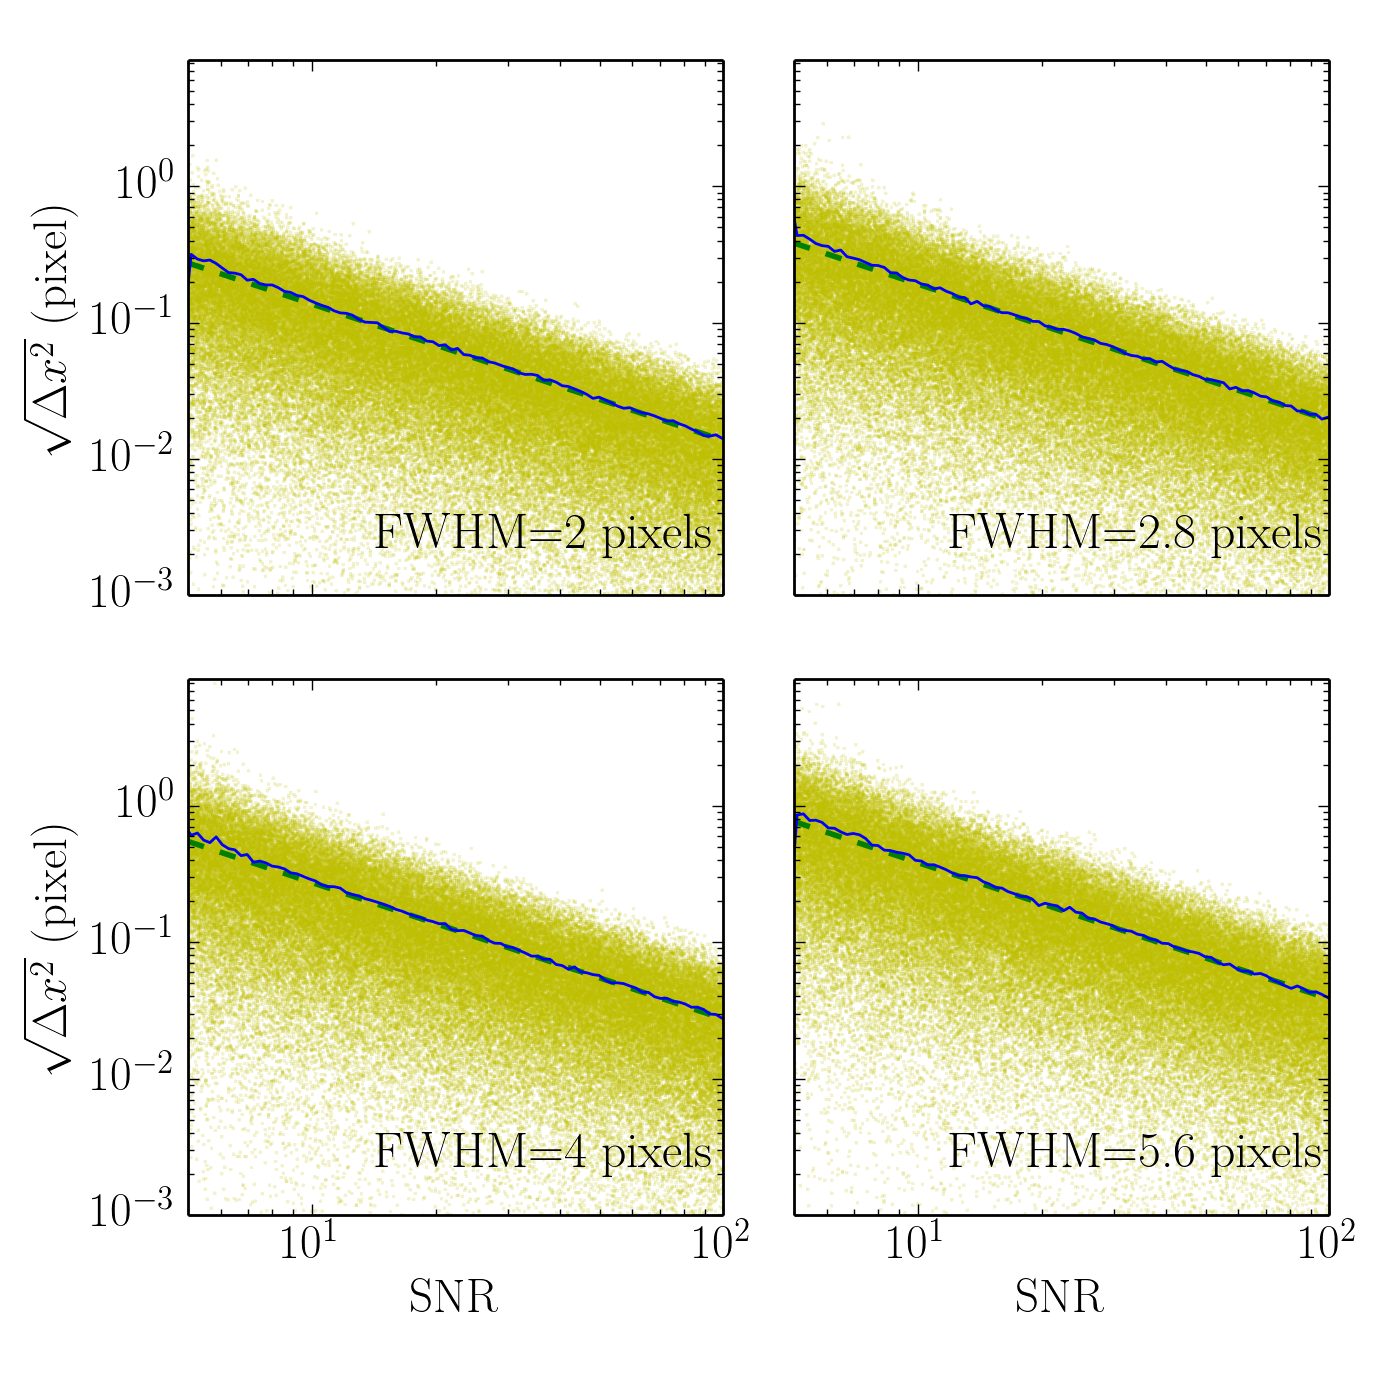
\includegraphics[width=\linewidth]{snr_psffitting.png}
\endminipage
\caption{Scatter plots showing the relation between error in centroid measurement
from fitting the exact PSF model to the stars and the signal-to-noise ratio of stars,
with FWHM of : 2 (upper left), 2.8 (upper right), 4 (lower left), and 5.6 (lower right)
pixels. In each scatter plot, the blue solid line represents the root-mean-squared-error, and the green dashed line represents CRLB.}\label{1}
\end{figure}

\begin{figure}[!htb]
\minipage{.8\textwidth}
  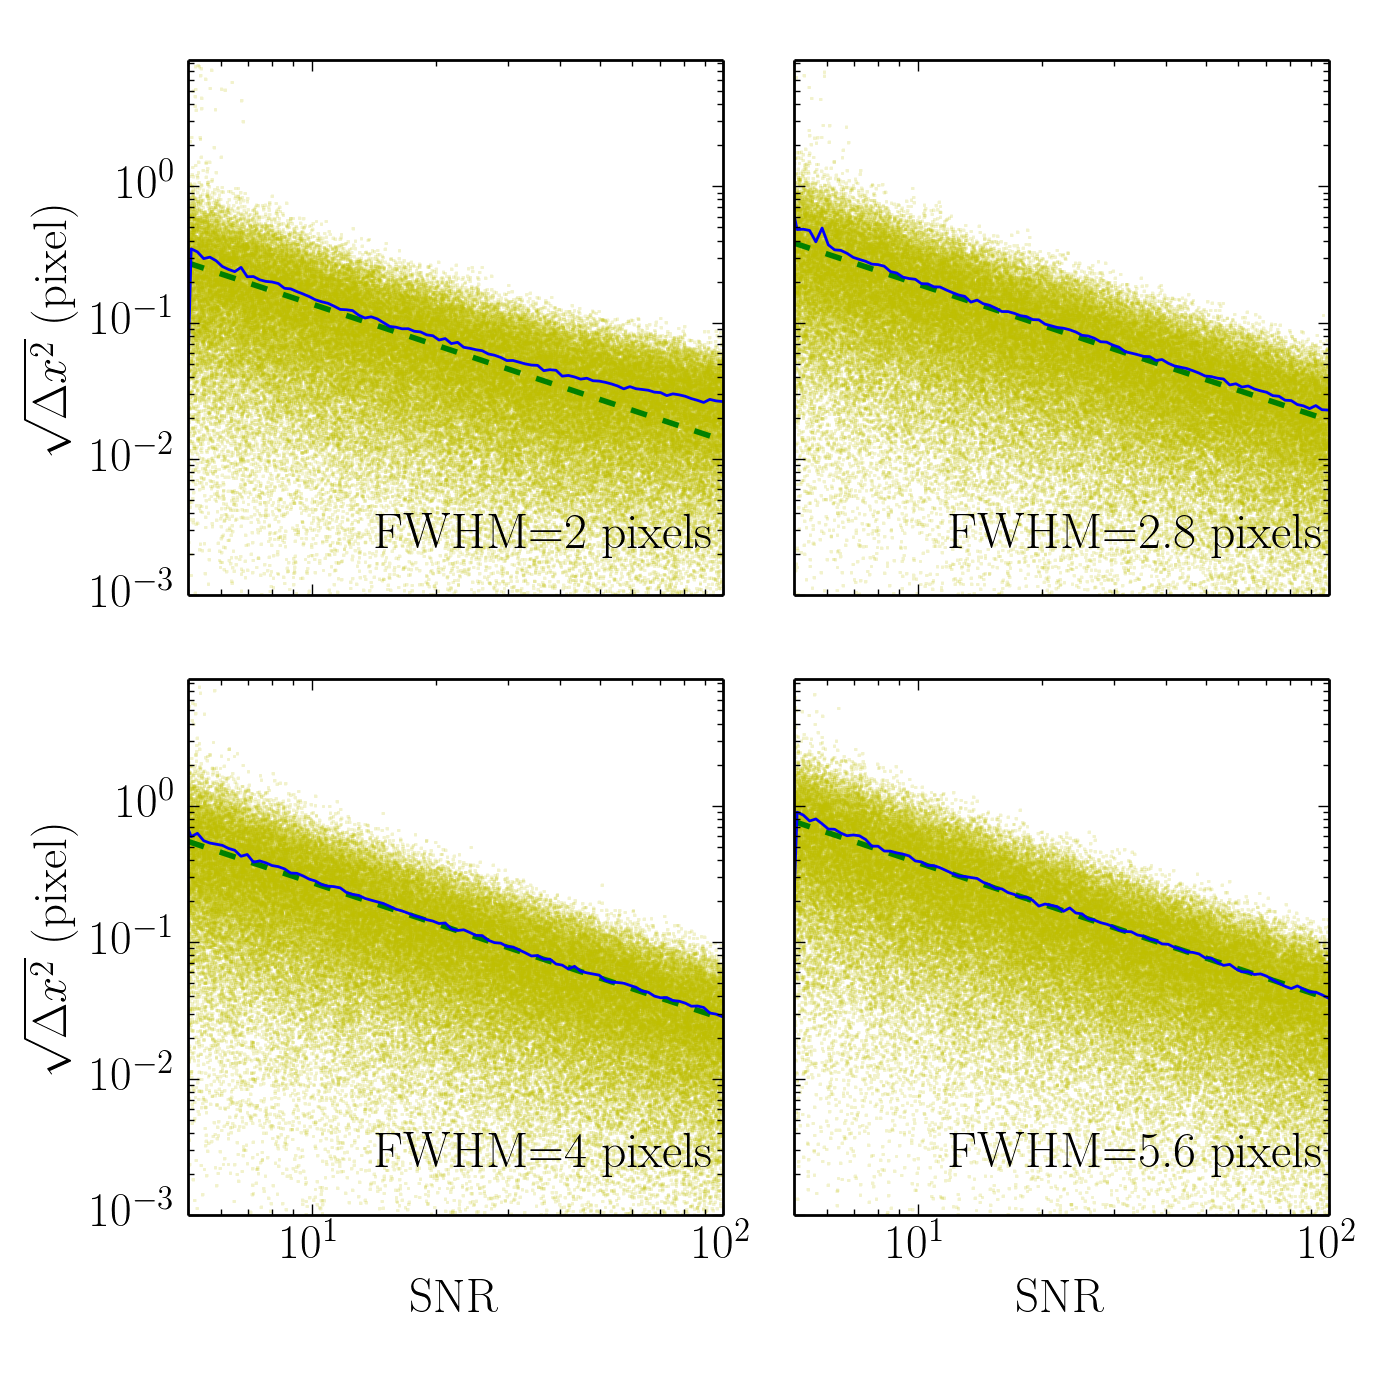
\includegraphics[width=\linewidth]{snr_psfpoly.png}
\endminipage
\caption{Scatter plots showing the relation between error in centroid
measurement from the PSF-based 3$\times$3 polynomial method and the signal-to-noise
ratio of stars, with FWHM of : 2 (upper left), 2.8 (upper right), 4 (lower left),
and 5.6 (lower right) pixels. In each scatter plot, the blue solid line represents the root-mean-squared-error, and the green dashed line represents CRLB.}\label{2}
\end{figure}

\begin{figure}[!htb]
\minipage{.8\textwidth}
  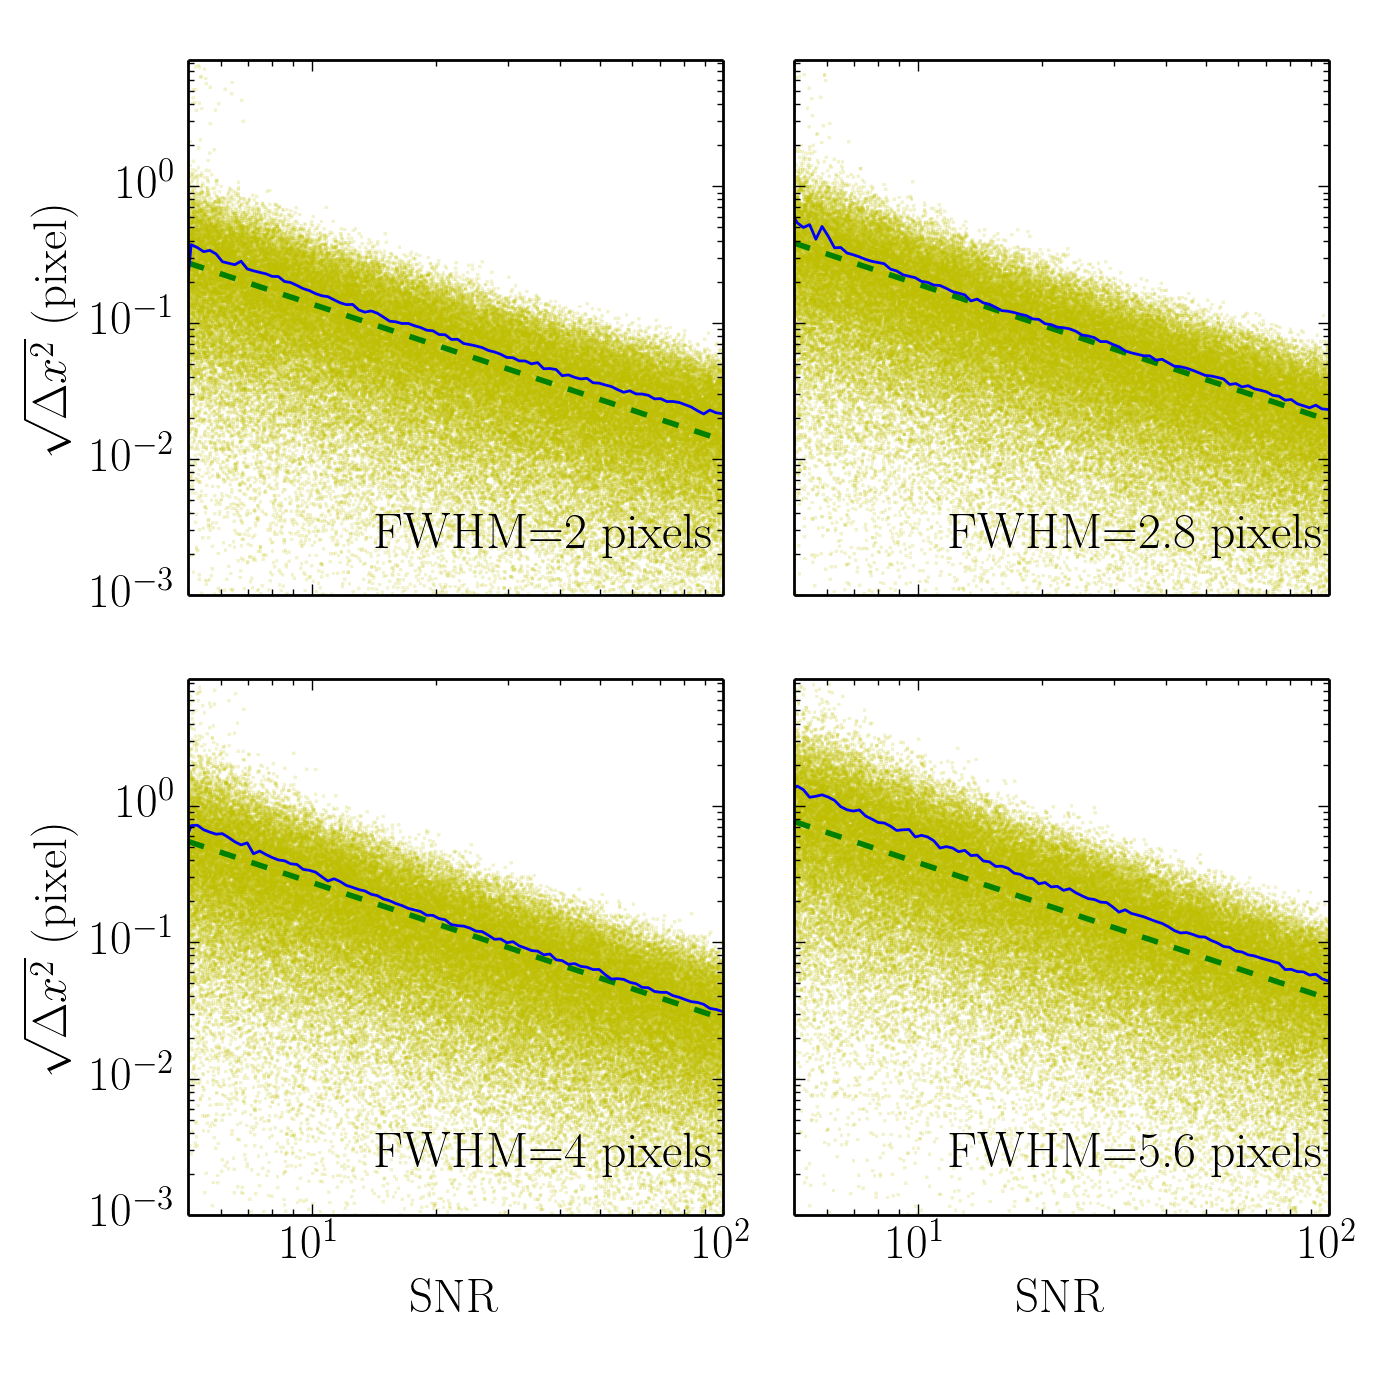
\includegraphics[width=\linewidth]{snr_psfpix28poly.png}
\endminipage
\caption{Scatter plots showing the relation between error in centroid measurement from the 3$\times$3 polynomial centroiding and the signal-to-noise ratio of stars, with FWHM of : 2 (upper left), 2.8 (upper right), 4 (lower left), and 5.6 (lower right) pixels. In each scatter plot, the blue solid line represents the root-mean-squared-error, and the green dashed line represents CRLB.}\label{3}
\end{figure}

\begin{figure}[!htb]
\minipage{.8\textwidth}
  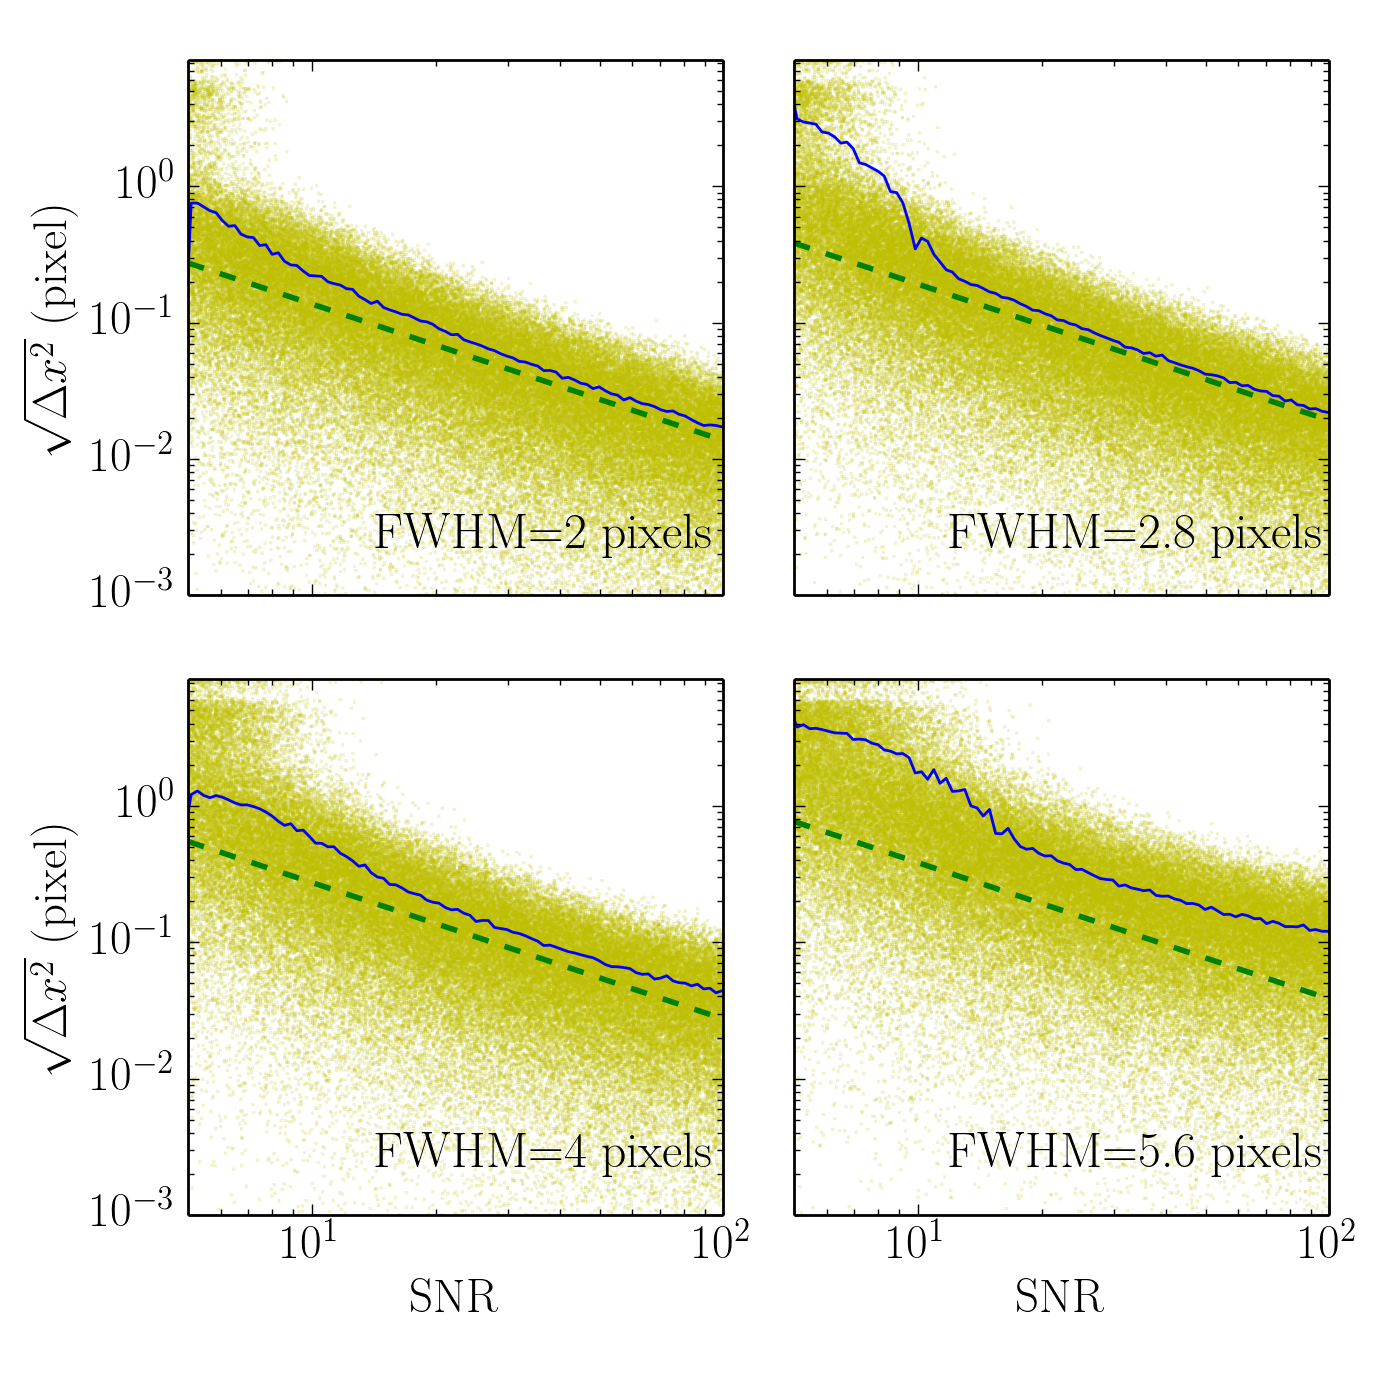
\includegraphics[width=\linewidth]{snr_moment.png}
\endminipage
\caption{Scatter plots showing the relation between error in centroid measurement from the 7$\times$7 moment method and the signal-to-noise ratio of stars, with FWHM of : 2 (upper left), 2.8 (upper right), 4 (lower left), and 5.6 (lower right) pixels. In each scatter plot, the blue solid line represents the root-mean-squared-error, and the green dashed line represents CRLB.}\label{4}
\end{figure}

%%%%%%%%%%%%%%%%%%%%%%%%%%%%%%%%%%%%%%%%%%%%%%%%%%%%%%%%%%%%%%%%%%%%%%%%%%% FWHM PLOTS %%%%%%%%%%%%%%%%%%%%%%%%%%%%%%%%%%%%%%%%%%

\begin{figure}[!htb]
\minipage{.8\textwidth}
  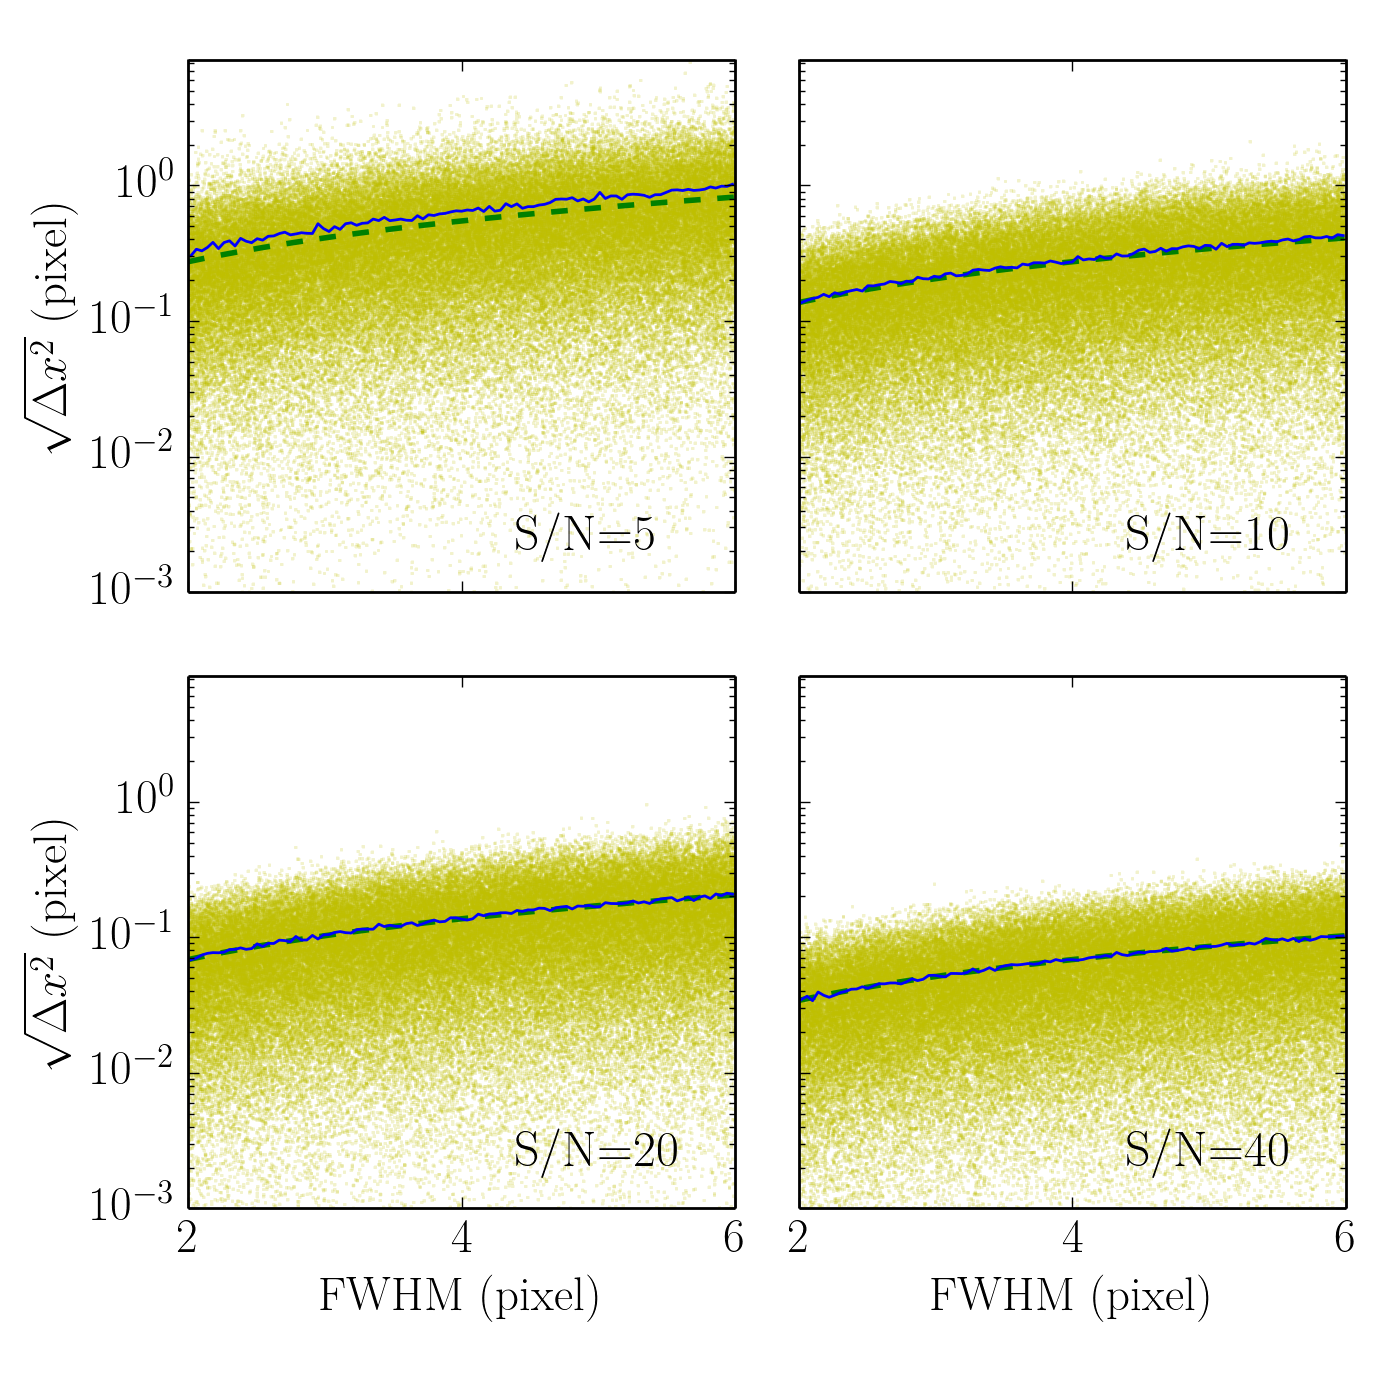
\includegraphics[width=\linewidth]{fwhm_psf.png}
\endminipage
\caption{Scatter plots showing the relation between error in centroid measurement
from fitting the exact PSF model and FWHM of stars, with SNR  of : 5 (upper left),
10 (upper right), 20 (lower left), and 40 (lower right). In each scatter plot,
the blue solid
 line represents the root-mean-squared-error, and the green dashed line represents CRLB.}\label{5}
\end{figure}

\begin{figure}[!htb]
\minipage{.8\textwidth}
  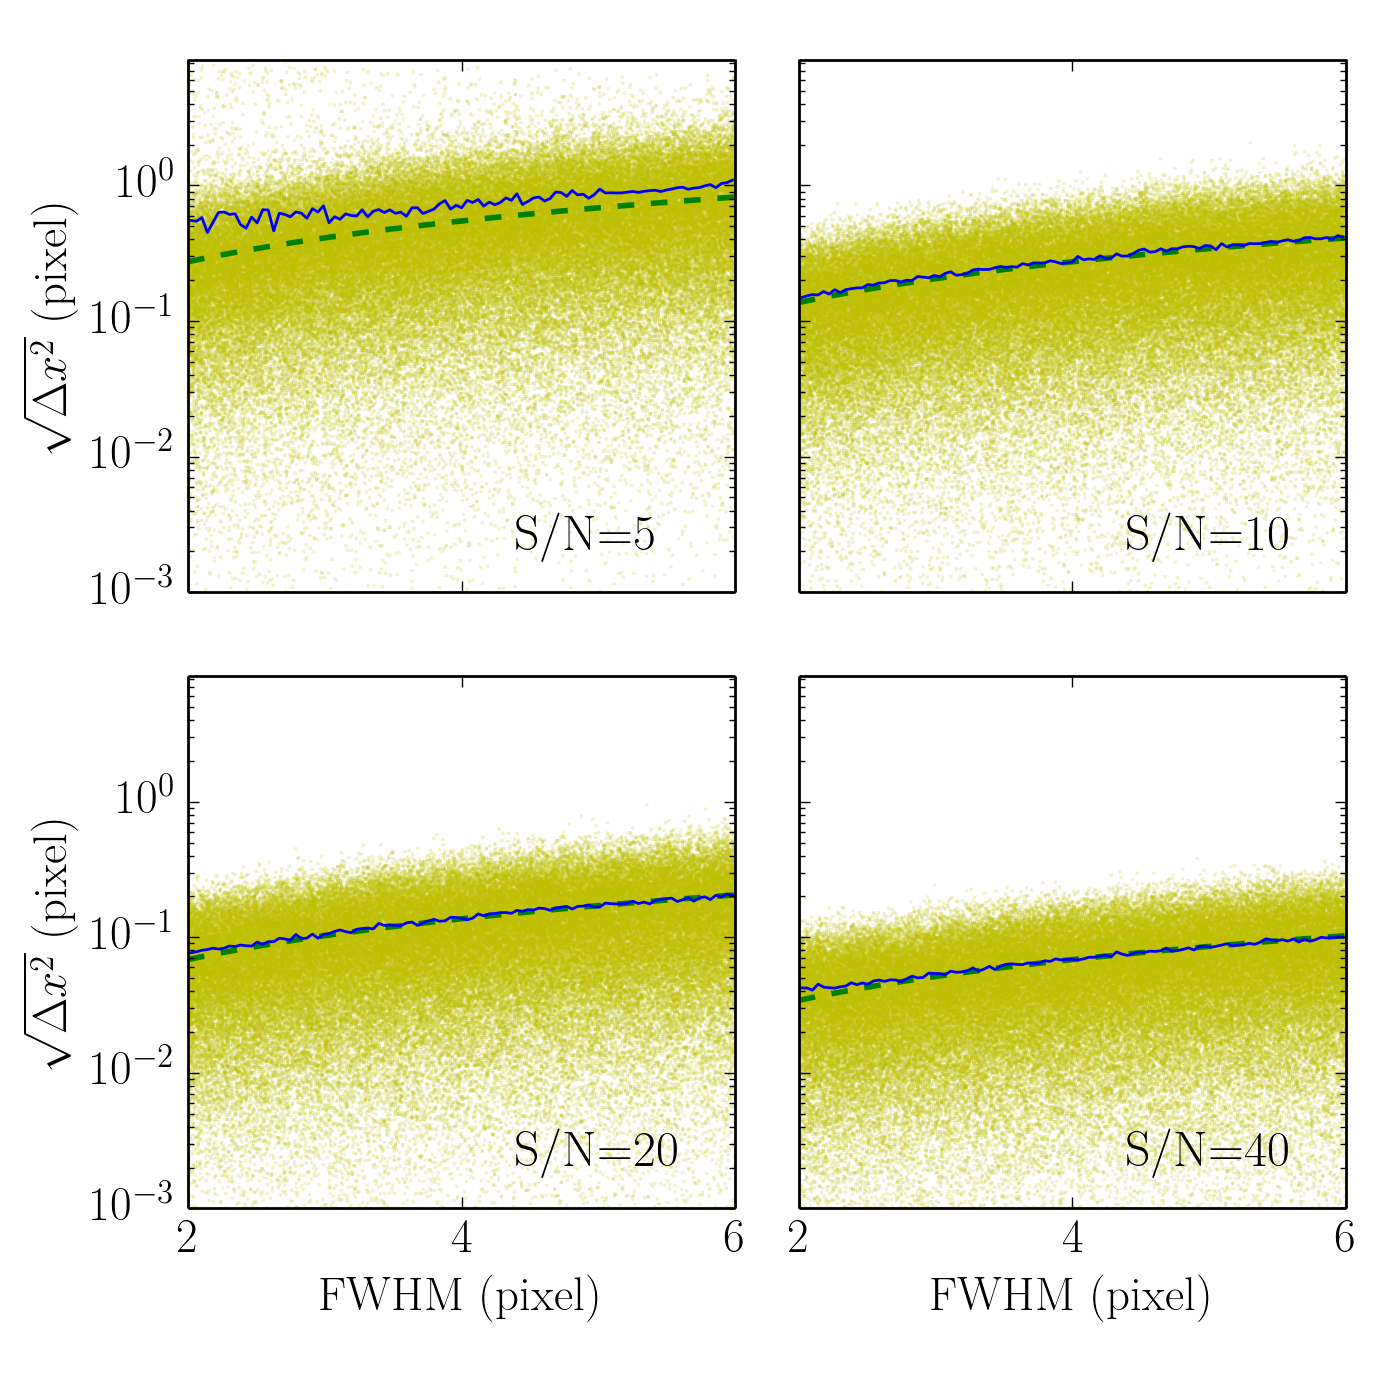
\includegraphics[width=\linewidth]{fwhm_psfpoly.png}
\endminipage
\caption{Scatter plots showing the relation between error in centroid measurement
from the PSF-based 3$\times$3 polynomial method and FWHM of stars, with SNR  of : 5 (upper left),
10 (upper right), 20 (lower left), and 40 (lower right). In each scatter plot, the blue solid
 line represents the root-mean-squared-error, and the green dashed line represents CRLB.}\label{6}
\end{figure}

\begin{figure}[!htb]
\minipage{.8\textwidth}
  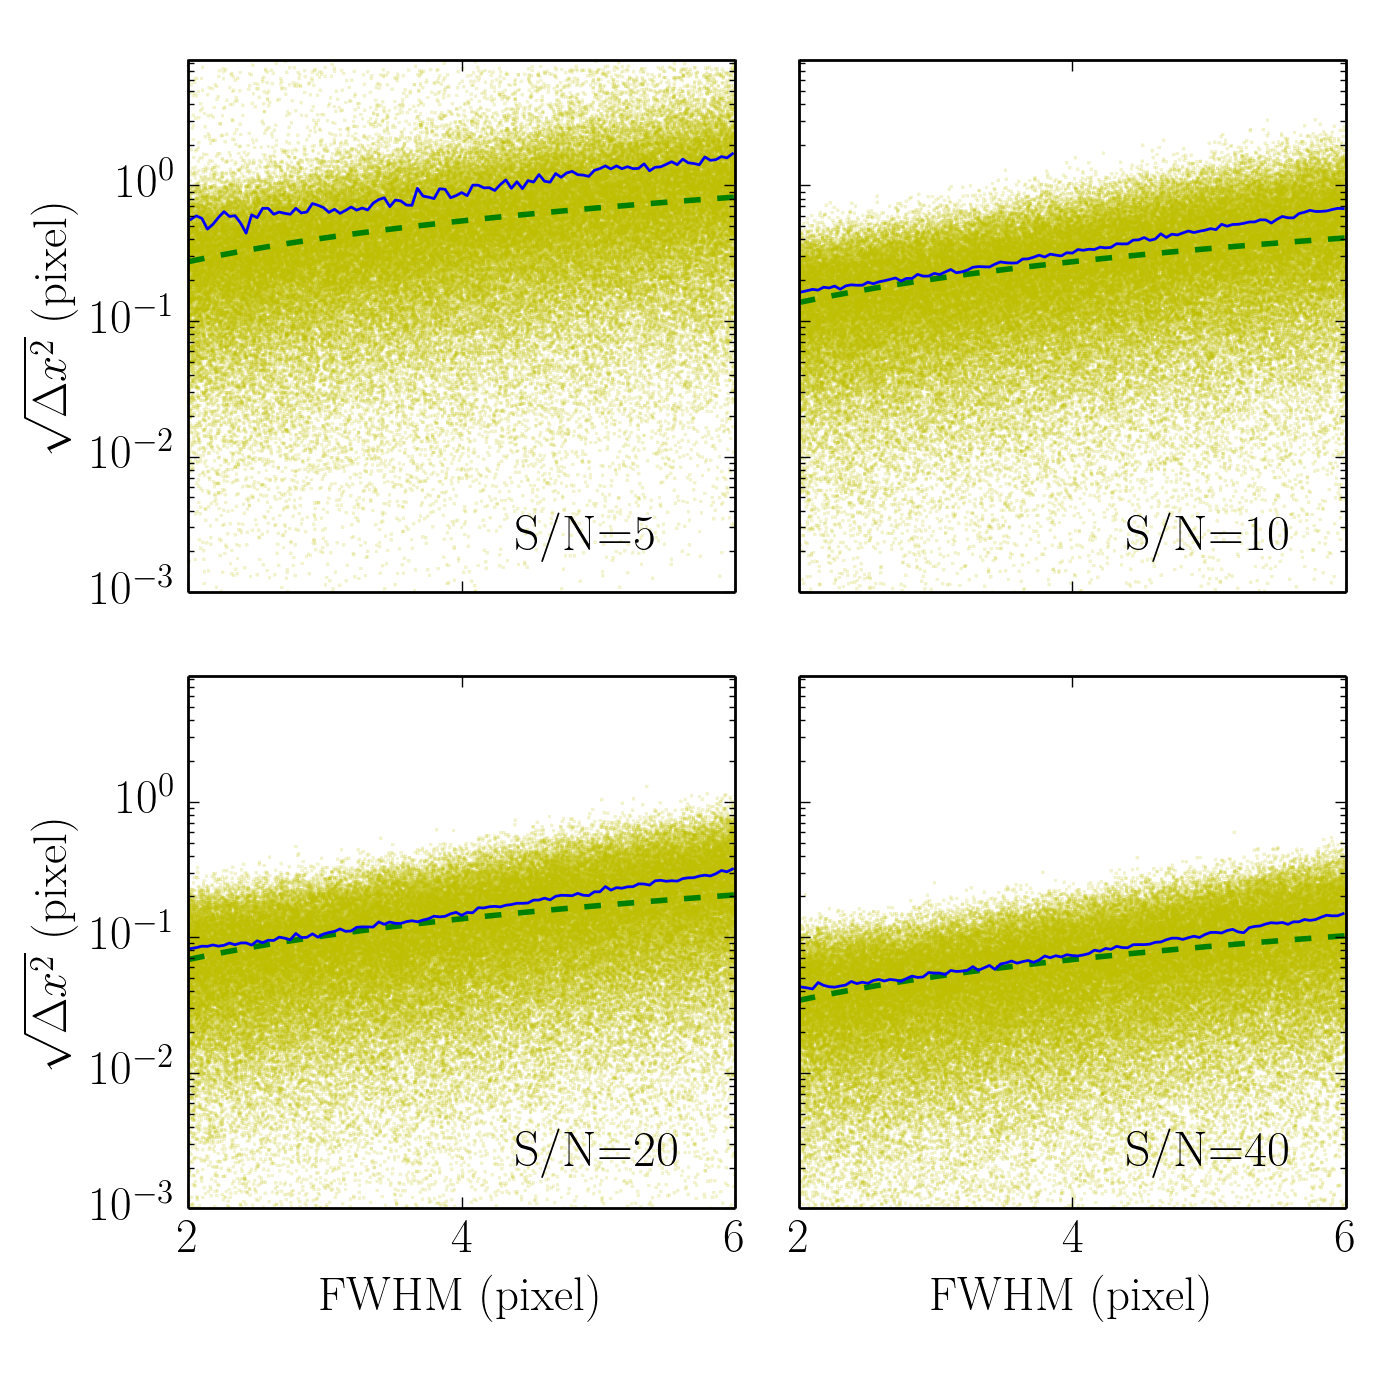
\includegraphics[width=\linewidth]{fwhm_psfpix28poly.png}
\endminipage
\caption{Scatter plots showing the relation between error in centroid measurement
from the 3$\times$3 polynomial centroiding and FWHM of stars, with SNR  of 
: 5 (upper left), 10 (upper right), 20 (lower left), and 40 (lower right). In each
scatter plot, the blue solid
 line represents the root-mean-squared-error, and the green dashed line represents CRLB.}\label{7}
\end{figure}

\begin{figure}[!htb]
\minipage{.8\textwidth}
  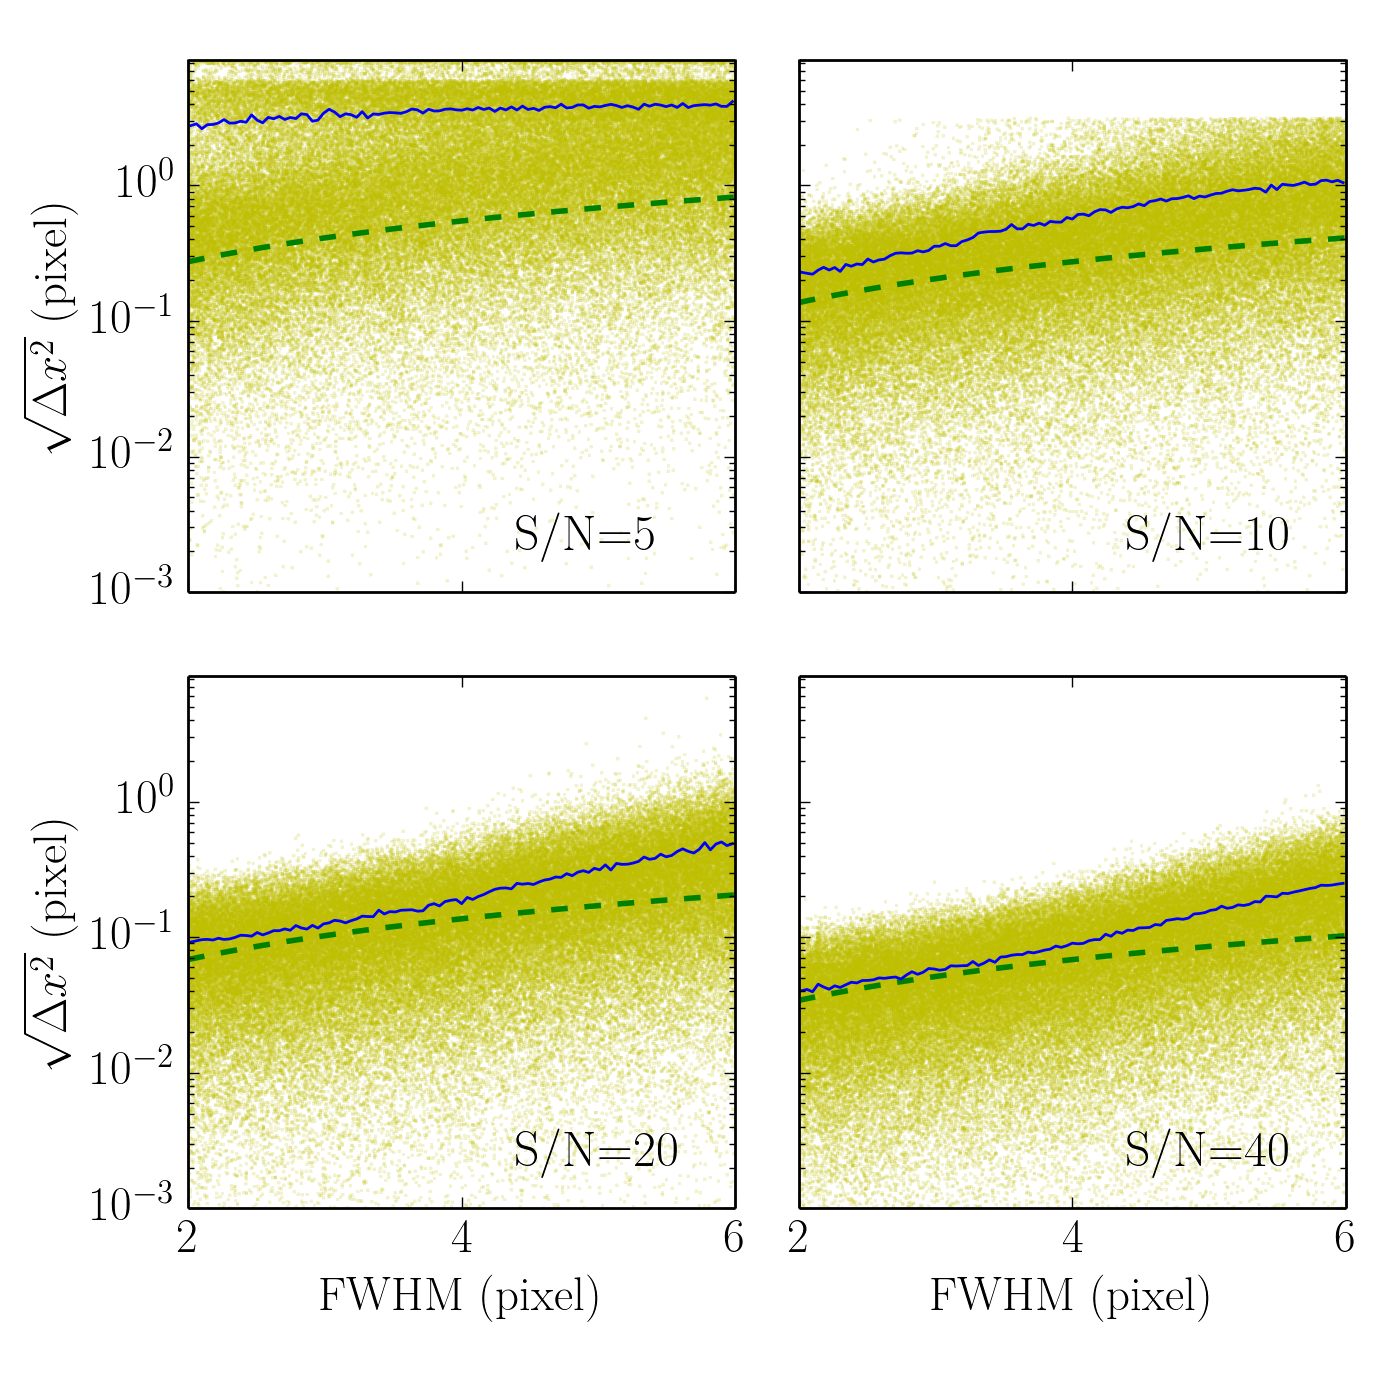
\includegraphics[width=\linewidth]{fwhm_moment.png}
\endminipage
\caption{Scatter plots showing the relation between error in centroid measurement
from the 7$\times$7 moment method and FWHM of stars, with SNR of : 5 (upper left),
10 (upper right), 20 (lower left), and 40 (lower right). In each scatter plot, 
the blue solid
 line represents the root-mean-squared-error, and the green dashed line represents CRLB.}\label{8}
\end{figure}

\end{document}
